%!TEX root = ../../thesis.tex

The leading and subleading contributions to the top background are the \ttbar and 
\HepProcess{\PW\Ptop} processes, respectively. These are irreducible backgrounds, in that 
they both exhibit the opposite-sign dilepton + \met experimental signature. This occurs via 
top decays $\text{BR}\parenths{\HepProcess{\Ptop \HepTo \PW\Pbottom}} \approx 100\%$ 
(occurs before hadronisation) and leptonic \PW boson decays.

Considering \HepProcess{\ttbar \HepTo \PW\PW\Pbottom\Pbottom} and \HepProcess{\PW\Ptop 
\HepTo \PW\PW\Pbottom}, it is clear that top events feature one or two \Pbottom-jets. This 
motivates the jet binning of the \HWW analysis (see \Figure~\ref{fig:sel:njets}), using 
jets with a \pt threshold of \unit{25(30)}{\GeV} in the central (forward) region (see 
\Section~\ref{sec:objects:jets}). The top background is further discriminated by counting 
the number of \Pbottom-tagged jets with \unit{$\pt > 20$}{\GeV} in the central region, 
using an algorithm with a tagging efficiency of 85\% (see \Section~\ref{sec:objects:bjets}).
In the 1-jet and \twojet bins, the top background is suppressed by vetoing events with 
\Pbottom-tagged jets.

\ttbar, \HepProcess{\PW\Ptop} and $s$-channel single top are modelled by 
\meps{\powhegbox}{\pythia{6}}, while $t$-channel single top is modelled by 
\meps{\acermc}{\pythia{6}}. However, the jet binning and \Pbottom-tagged jet veto 
introduce large modelling uncertainties, and so data-driven techniques are used to 
estimate this background.



\subsection{0-jet bin estimation}
\label{sec:top:0j}

In the 0-jet bin, the top background is very small because both \Pbottom-jets must fail the 
jet selection. It is estimated by the data-driven \textit{jet veto survival probability 
method} since the jet veto efficiency $\epsilon_0$ has large uncertainties.

An extended signal region (ESR) is defined by the pre-selection in 
\Section~\ref{sec:selection:presel}, with an additional $\dphill < 2.8$ criterion to 
suppress the \DYtt background. The aim is to estimate the number of events in the ESR 
passing the jet veto $N_{\text{top}}^{\text{pred,ESR,0j}}$, and then extrapolate to the 
0-jet signal region (SR) with MC
\begin{equation}
	N_{\text{top}}^{\text{pred,SR,0j}} &= \alpha_{\text{top}}^{\text{0j}} \cdot \epsilon_{\text{0,top}}^{\text{pred,ESR}} \cdot \parenths{N^{\text{data,ESR}} - N_{\text{non-top}}^{\text{pred,ESR}}} \\
	\alpha_{\text{top}}^{\text{0j}} &= N_{\text{top}}^{\text{MC,SR,0j}} / N_{\text{top}}^{\text{MC,ESR,0j}}
\end{equation}
where $\epsilon_{0}$ is the jet veto efficiency. \Figure~\ref{fig:sel:njets} shows that, 
after pre-selection, top dominates the \emch/\mech channels, but \DYll dominates the 
\eech/\mmch channels. For this reason, the top normalisation is derived from a combined 
\emch{}+\mech channel and extrapolated to each \emch/\mech/\eech/\mmch SR.

The ESR is dominated by \ttbar events featuring two \Pbottom-jets. Since each 
\Pbottom-quark originates from the decay of a top quark, the kinematic distributions of the 
two jets are similar. Thus, it is possible to make the approximation 
$\epsilon_{\text{0,top}} = \epsilon_{\text{1,top}}^2$, where $\epsilon_{1}$ is the veto 
efficiency of a second jet. This $\epsilon_{\text{1,top}}$ is experimentally measured in a 
high-purity top control region (CR) and is used to correct the $\epsilon_{\text{0,top}}$ 
modelled by MC in the ESR:
\begin{equation}
	\epsilon_{\text{0,top}}^{\text{pred,ESR}} &= \epsilon_{\text{0,top}}^{\text{MC,ESR}} \parenths{\frac{\epsilon_{1}^{\text{data,CR}}}{\epsilon_{\text{1,top}}^{\text{MC,CR}}}}^{\!\!2} \,. \label{eq:jvsp}
\end{equation}
The top CR requires at least one \Pbottom-tagged jet with \unit{$\pt > 25$}{\GeV}, relative 
to the ESR. Then $\epsilon_{\text{1,top}}^{\text{data,CR}}$ is measured by counting the 
fraction of CR events with zero additional jets. These are defined as jets with 
$\Delta R > 1$ from the highest scoring \Pbottom-tagged jet (see \Figure~\ref{fig:top:jvsp}). It is found that (\ref{eq:jvsp}) is not invalidated by contributions from other top 
processes and jets other than the two \Pbottom-jets.

\begin{figure}[t]
	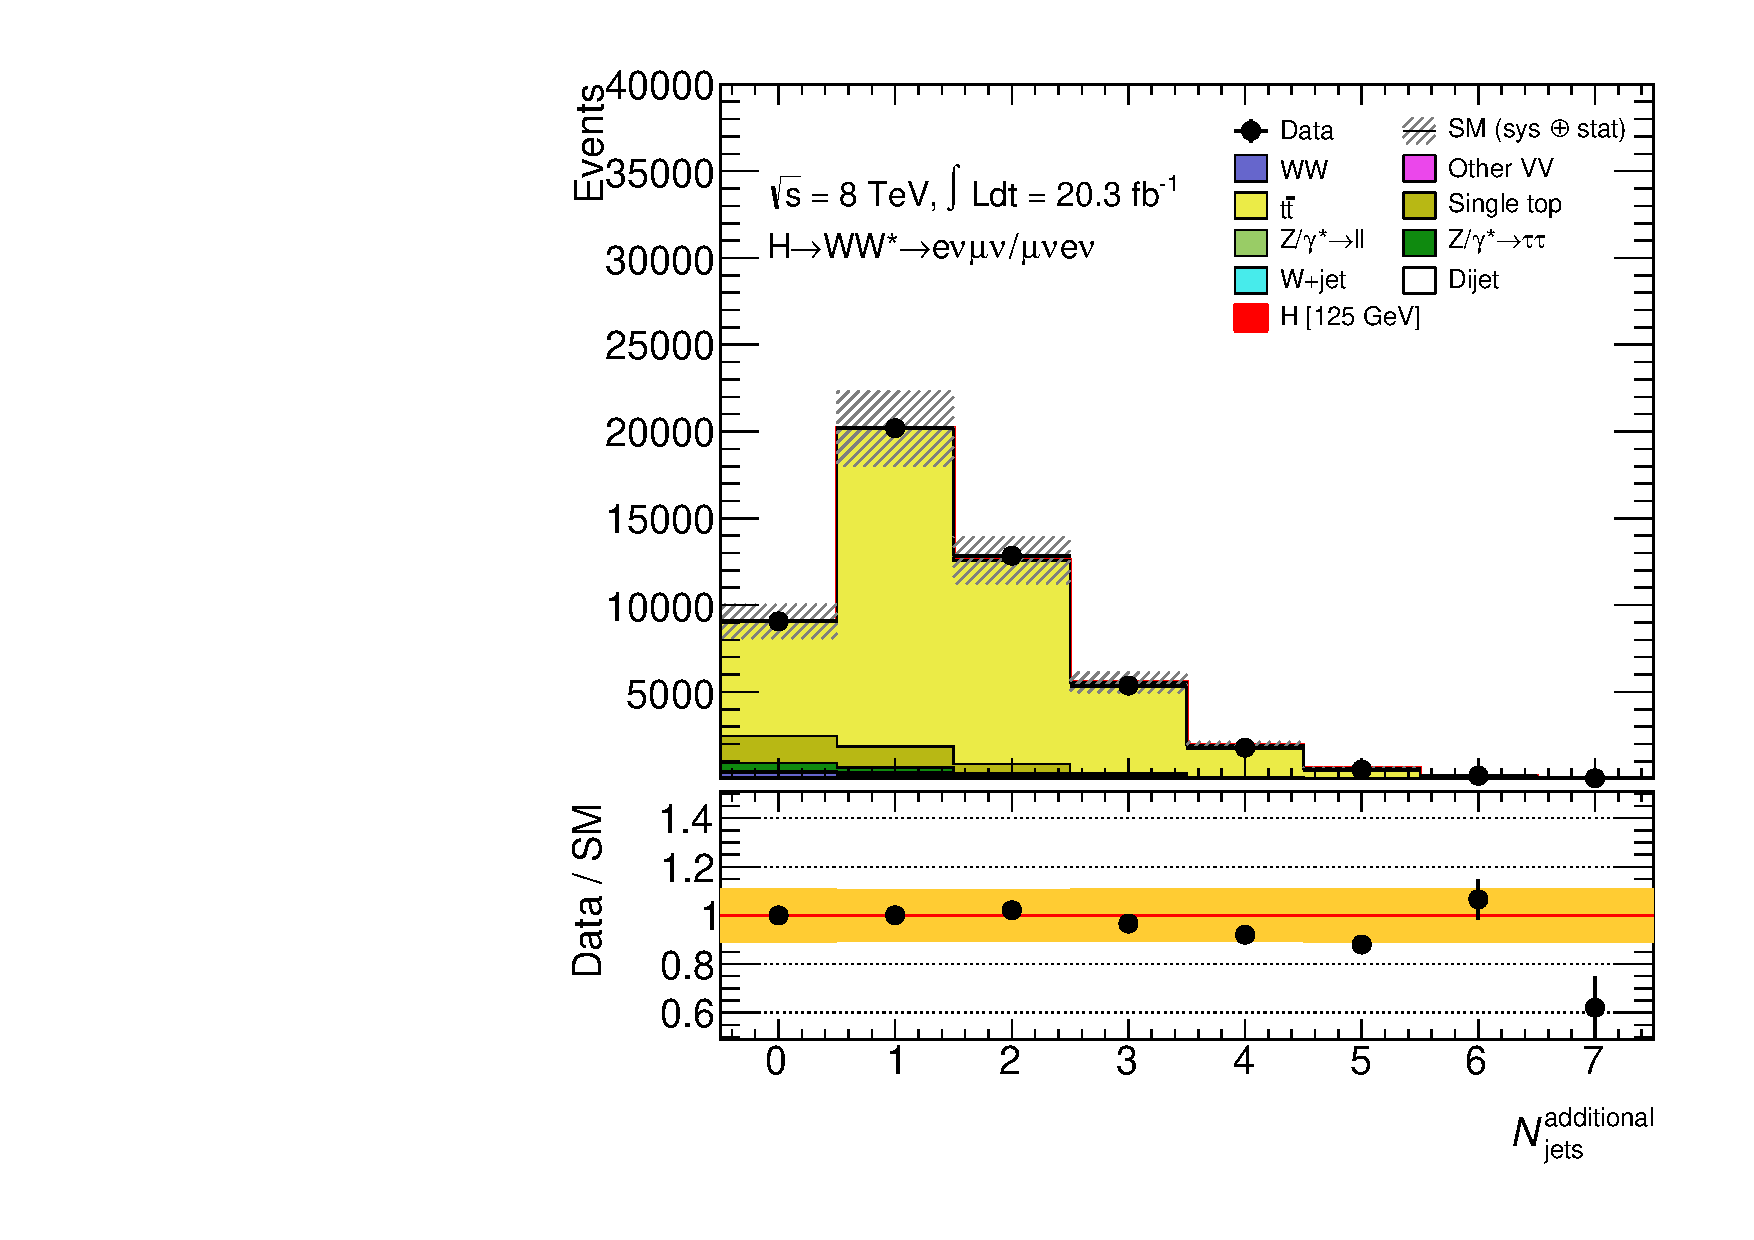
\includegraphics[width=0.495\textwidth]{tex/backgrounds/emme_CutTopControl_AddTrackMET_nJets_probing_mh125_lin}
	\hfill
	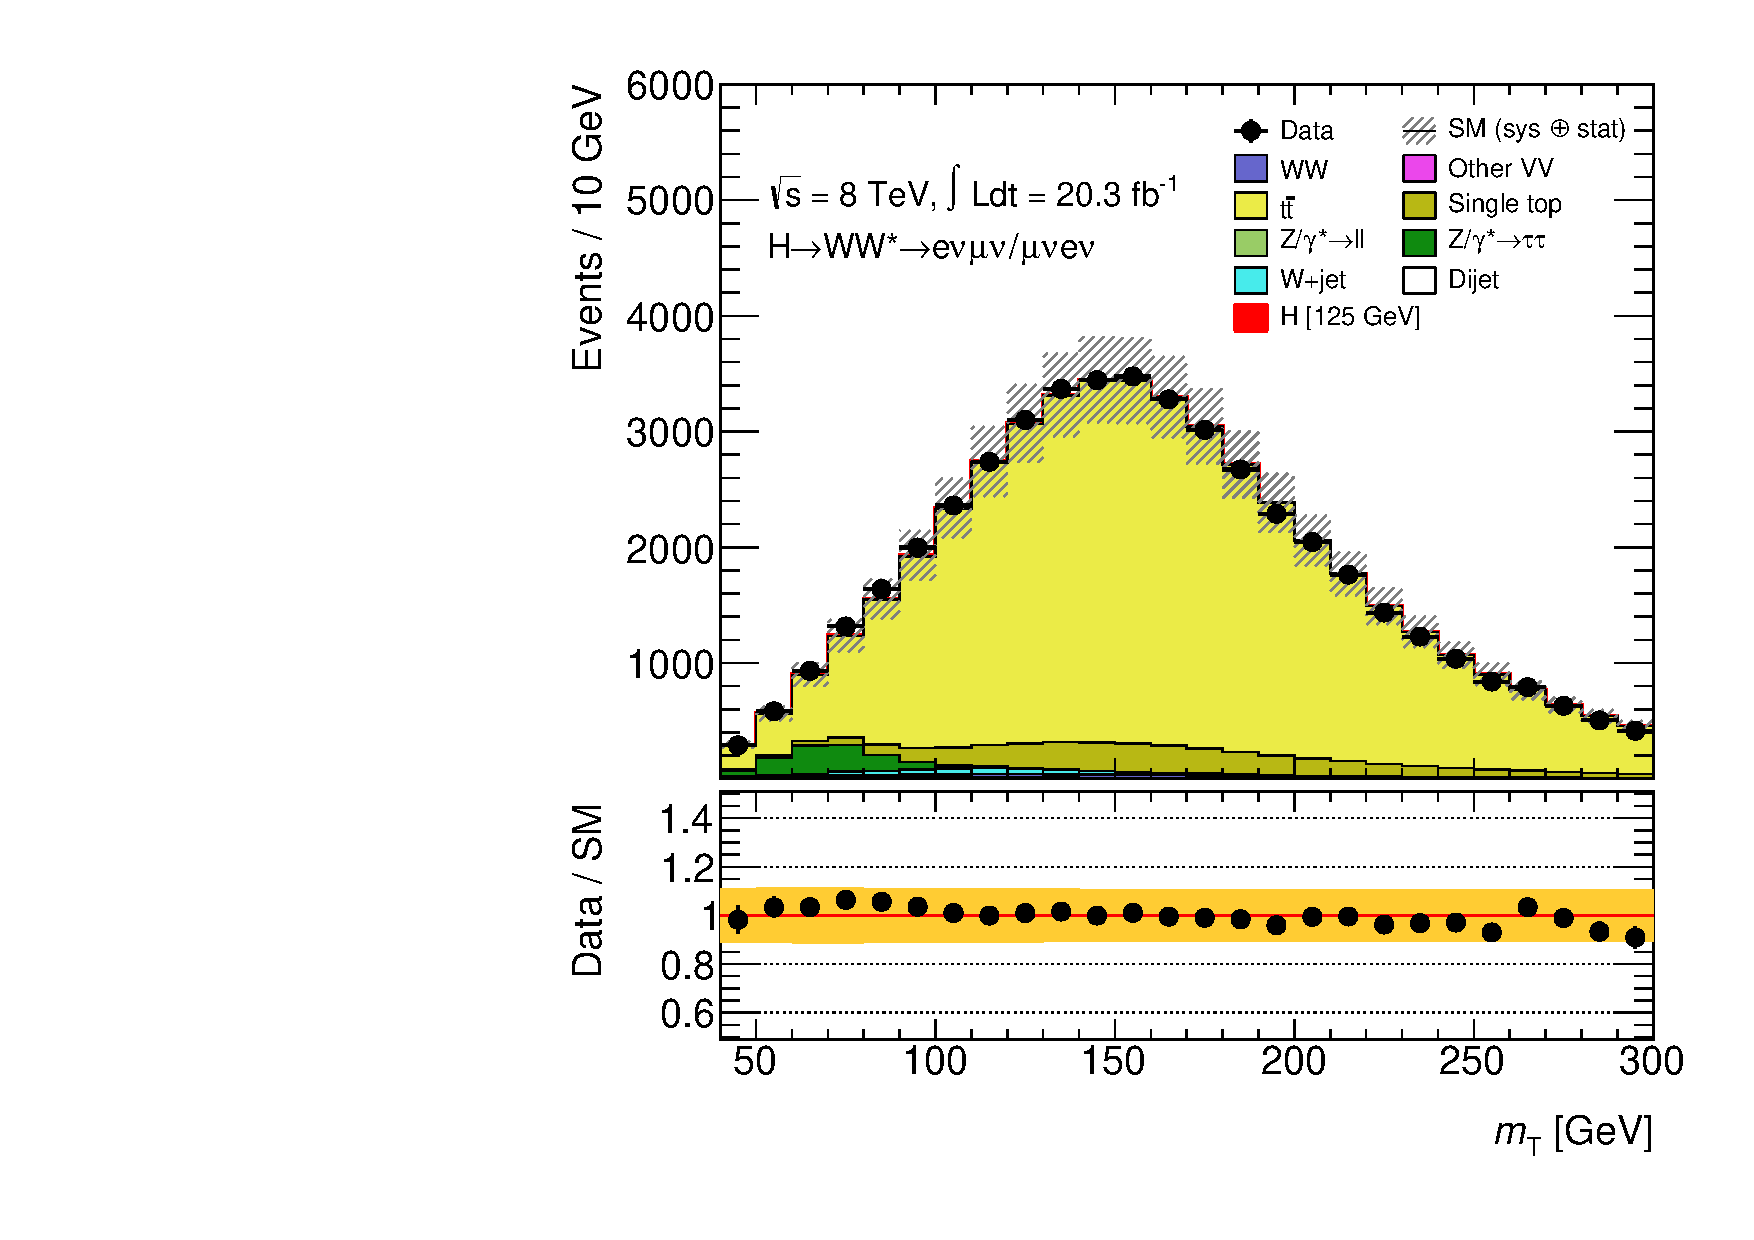
\includegraphics[width=0.495\textwidth]{tex/backgrounds/emme_CutTopControl_AddTrackMET_MT_TrackHWW_Clj_mh125_lin}
	\caption{The number of additional jets (left) and the \mt distribution (right) in the 
	top control region used by the jet veto survival probability method. The fraction of 
	events with zero additional jets is $\epsilon_{\text{1,top}}^{\text{data,CR}}$, as 
	described in the text.}
	\label{fig:top:jvsp}
\end{figure}

The total uncertainties in the expected 0-jet top background is \about8.2\%, dominated by 
theoretical uncertainties in the extrapolation $\alpha_{\text{top}}^{\text{0j}}$ and 
JES/JER uncertainties in the predicted jet veto efficiency 
$\epsilon_{\text{0,top}}^{\text{pred,ESR}}$.

To estimate the top background in 0-jet regions other than the SR, the method is viewed as 
providing a simple data-driven normalisation factor. This is equivalent to neglecting the 
extrapolation uncertainties, but is helpful when plotting observables. The normalisation 
factor is measured to be \stat{1.115}{0.031}\todo{update}.



\subsection{1-jet bin estimation}
\label{sec:top:1j}

In the 1-jet bin, the top background is suppressed by removing events with a 
\Pbottom-tagged jet with \unit{$\pt > 20$}{\GeV}. Since the \Pbottom-tagging efficiency is 
associated with large uncertainties, the data-driven \textit{jet \Pbottom-tagging 
efficiency extrapolation method} is used to estimate this background.

An extended signal region (ESR) is defined by the pre-selection in 
\Section~\ref{sec:selection:presel}. Since it is the $\njets = 1$ selection and the 
\Pbottom-tagged jet veto that introduce the largest uncertainties to this background, the 
aim of the method is to estimate the number of events accepted by these cuts 
$N_{\text{top}}^{\text{pred,ESR,1j0\Pbottom}}$, and then extrapolate to the 1-jet signal 
region (SR) with MC
\begin{equation}
	N_{\text{top}}^{\text{pred,SR,1j0\Pbottom}} &= \alpha_{\text{top}}^{\text{1j}} \cdot N_{\text{top}}^{\text{pred,ESR,1j0\Pbottom}} \\
	\alpha_{\text{top}}^{\text{1j}} &= N_{\text{top}}^{\text{MC,SR,1j0\Pbottom}} / N_{\text{top}}^{\text{MC,ESR,1j0\Pbottom}} \,.
\end{equation}
The top normalisation is derived from a combined \emch{}+\mech channel and extrapolated to 
each \emch/\mech/\eech/\mmch SR.

In order to estimate $N_{\text{top}}^{\text{pred,ESR,1j0\Pbottom}}$, the number of 1-jet 
events in the ESR with a \Pbottom-tagged jet $N^{\text{data,ESR,1j1\Pbottom}}$ is measured, 
which is highly pure in top events (see \Figure~\ref{fig:top:jbee})\todo{Add systematics to 
error band}. Then the non-top contamination is subtracted, and the \Pbottom-tagged jet 
selection is inverted using the expected \Pbottom-tagging efficiency 
$\varepsilon_{\Pbottom}^{\text{pred,ESR,1j}}$:
\begin{equation}
	N_{\text{top}}^{\text{pred,SR,1j0\Pbottom}} &= \alpha_{\text{top}}^{\text{1j}} \cdot \frac{1 - \varepsilon_{\Pbottom}^{\text{pred,ESR,1j}}}{\varepsilon_{\Pbottom}^{\text{pred,ESR,1j}}} \cdot \parenths{N^{\text{data,ESR,1j1\Pbottom}} - N_{\text{non-top}}^{\text{pred,ESR,1j1\Pbottom}}} \,.
\end{equation}
It should be emphasised that $\varepsilon_{\Pbottom}$ is a per-jet efficiency, rather than 
a per-event efficiency (\cf $\epsilon_0$). Also, $\varepsilon_{\Pbottom}$ is the average 
\Pbottom-tagging efficiency for a jet in a top event, and will include non-\Pbottom-jets 
(\ie it is a mixture of tagged \Pbottom-jets and mis-tagged other jets).

\begin{figure}[t]
	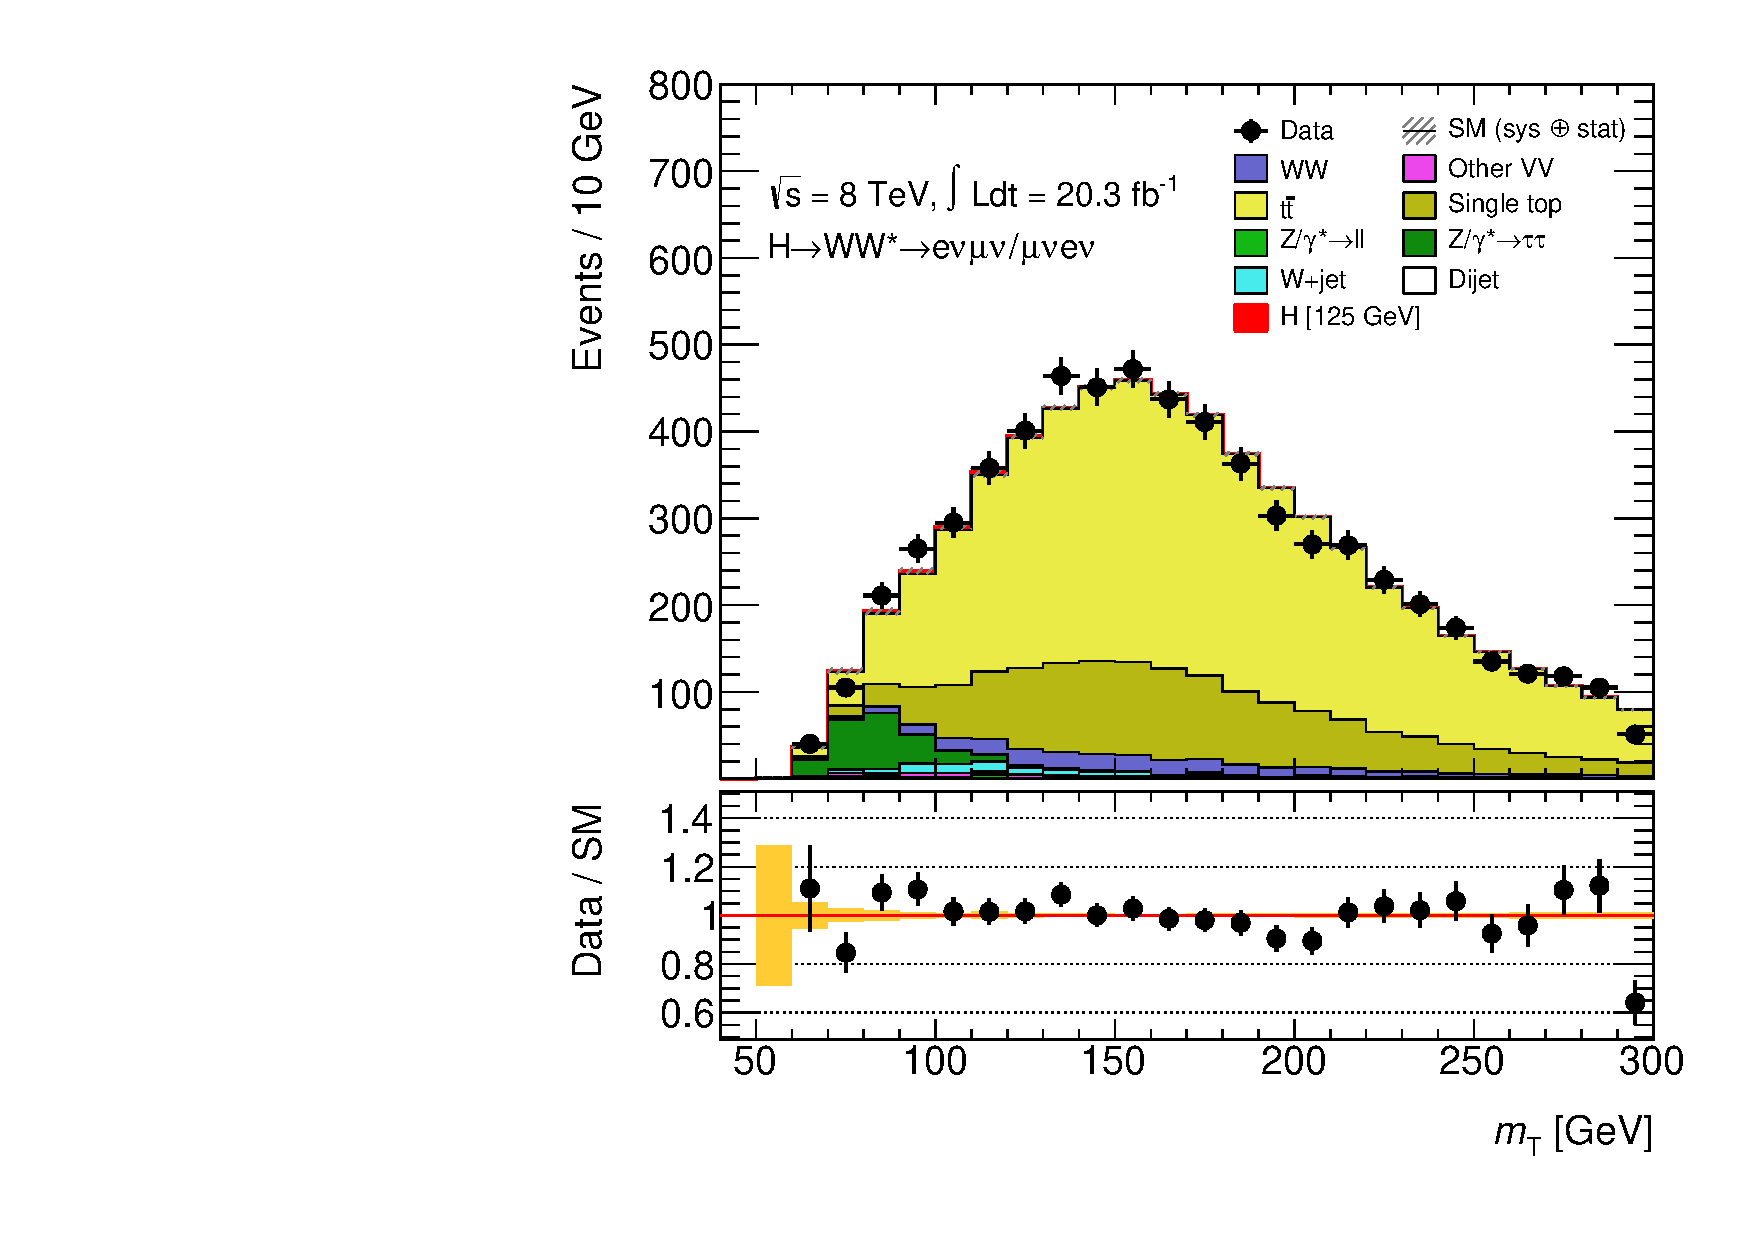
\includegraphics[width=0.495\textwidth]{tex/backgrounds/emme_CutMTW_1j_noSubBjet_Btagged_MT_TrackHWW_Clj_mh125_lin}
	\hfill
	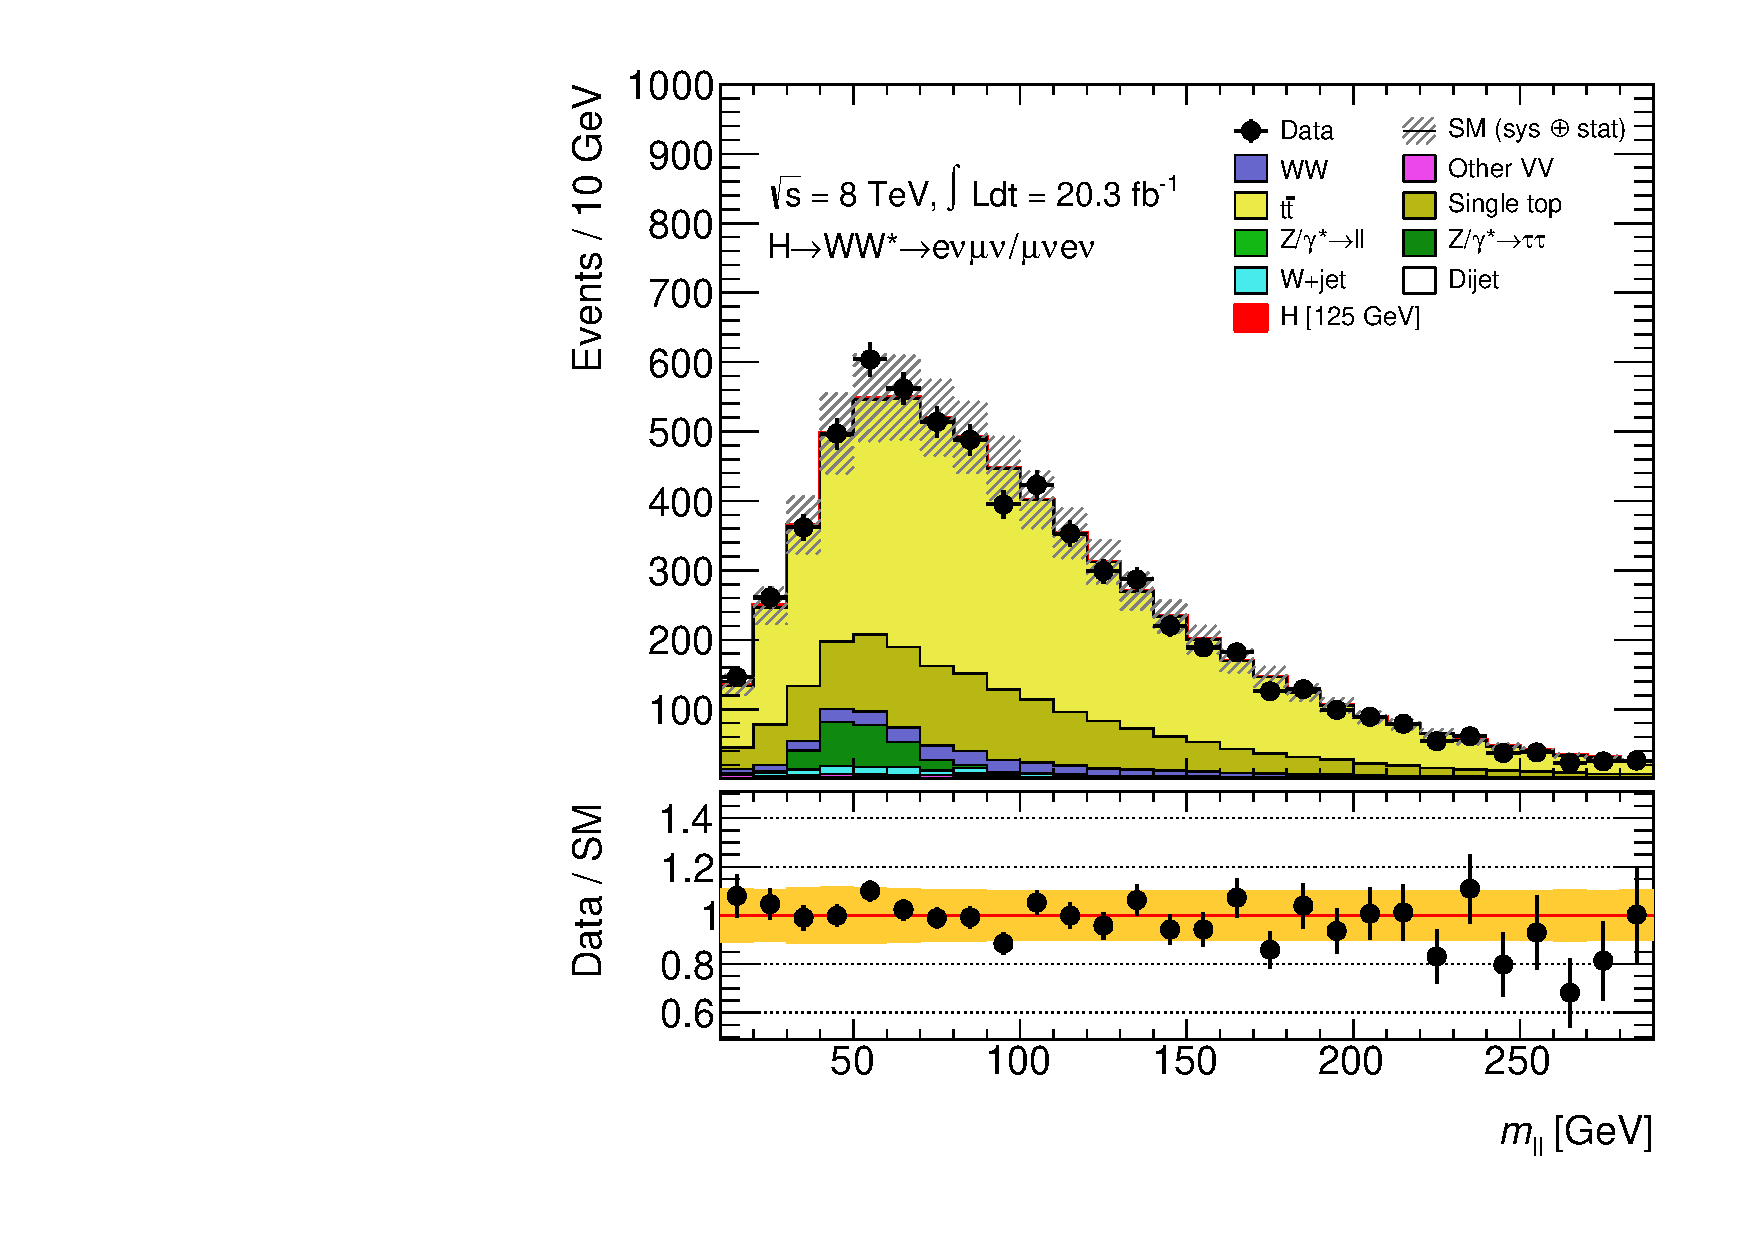
\includegraphics[width=0.495\textwidth]{tex/backgrounds/emme_CutMTW_1j_noSubBjet_Btagged_Mll_mh125_lin}
	\caption{The \mt (left) and \mll (right) distributions for events passing the 
	pre-selection and containing 1 jet and 1 \Pbottom-tagged jet. The jet \Pbottom-tagging 
	efficiency extrapolation method uses the top normalisation in this region and 
	extrapolates to events with 0 \Pbottom-tagged jets. Normalisation factors are applied.}
	\label{fig:top:jbee}
\end{figure}

The \Pbottom-tagging efficiency of jets in top events $\varepsilon_{\Pbottom}$ is measured 
in a high-purity top control region (CR). These events pass the pre-selection (minus the 
\corrtrackmet cut) and feature two jets, at least one of which is \Pbottom-tagged. 
$\varepsilon_{\Pbottom}$ is then measured using a tag-and-probe method, where the tag is a 
\Pbottom-tagged jet and the probe is the other jet. Since $\varepsilon_{\Pbottom}$ is 
measured in 2-jet events but applied to 1-jet events, an MC-based correction is applied to 
the measured \Pbottom-tagging efficiency
\begin{equation}
	\varepsilon_{\Pbottom}^{\text{pred,ESR,1j}} = \frac{\varepsilon_{\Pbottom}^{\text{MC,ESR,1j}}}{\varepsilon_{\Pbottom}^{\text{MC,CR,2j}}} \cdot \varepsilon_{\Pbottom}^{\text{data,CR,2j}} \,.
	\label{eq:top:jbee}
\end{equation}

The total uncertainty in the expected 1-jet top background is \about6.8\%, dominated by 
theoretical uncertainties in the MC-based correction to $\varepsilon_{\Pbottom}$ in 
(\ref{eq:top:jbee}).

To estimate the top background in 1-jet regions other than the SR, the method is viewed as 
providing a simple data-driven normalisation factor. This is equivalent to neglecting the 
extrapolation uncertainties, but is helpful when plotting observables. The normalisation 
factor is measured to be \stat{1.042}{0.025}\todo{update}.



\subsection{\twojet bin estimation}
\label{sec:top:2j}

As in the 1-jet bin, a veto on \Pbottom-tagged jets rejects the majority of the top 
background. However, even after this veto, top remains the largest background in the 
\twojet bin. Fortunately, this enables a top control region (CR) to be defined which 
includes the \Pbottom-tagged jet veto, greatly reducing the uncertainties due to 
\Pbottom-tagging efficiencies.

The top CR is defined in a high-\mll region, similarly to the \WW CRs in the 0-jet and 
1-jet bins. It is defined by the same criteria as the \twojet SR (minus the \mtautau, 
\dphill and \VH cuts), but the \mll cut is changed to \unit{$\mll > 80$}{\GeV}. The 
observed number of events is then extrapolated to the signal region (SR) using MC
\begin{equation}
	N_{\text{top}}^{\text{pred,SR}} &= \alpha_{\text{top}}^{\geq2\text{j}} \parenths{N^{\text{data,CR}} - N_{\text{non-top}}^{\text{pred,CR}}} \\
	\alpha_{\text{top}}^{\geq2\text{j}} &= N_{\text{top}}^{\text{MC,SR}} / N_{\text{top}}^{\text{MC,CR}} \,.
\end{equation}
The uncertainty is dominated by theoretical uncertainties in the extrapolation 
$\alpha_{\text{top}}^{\geq2\text{j}}$.

\begin{figure}[t]
	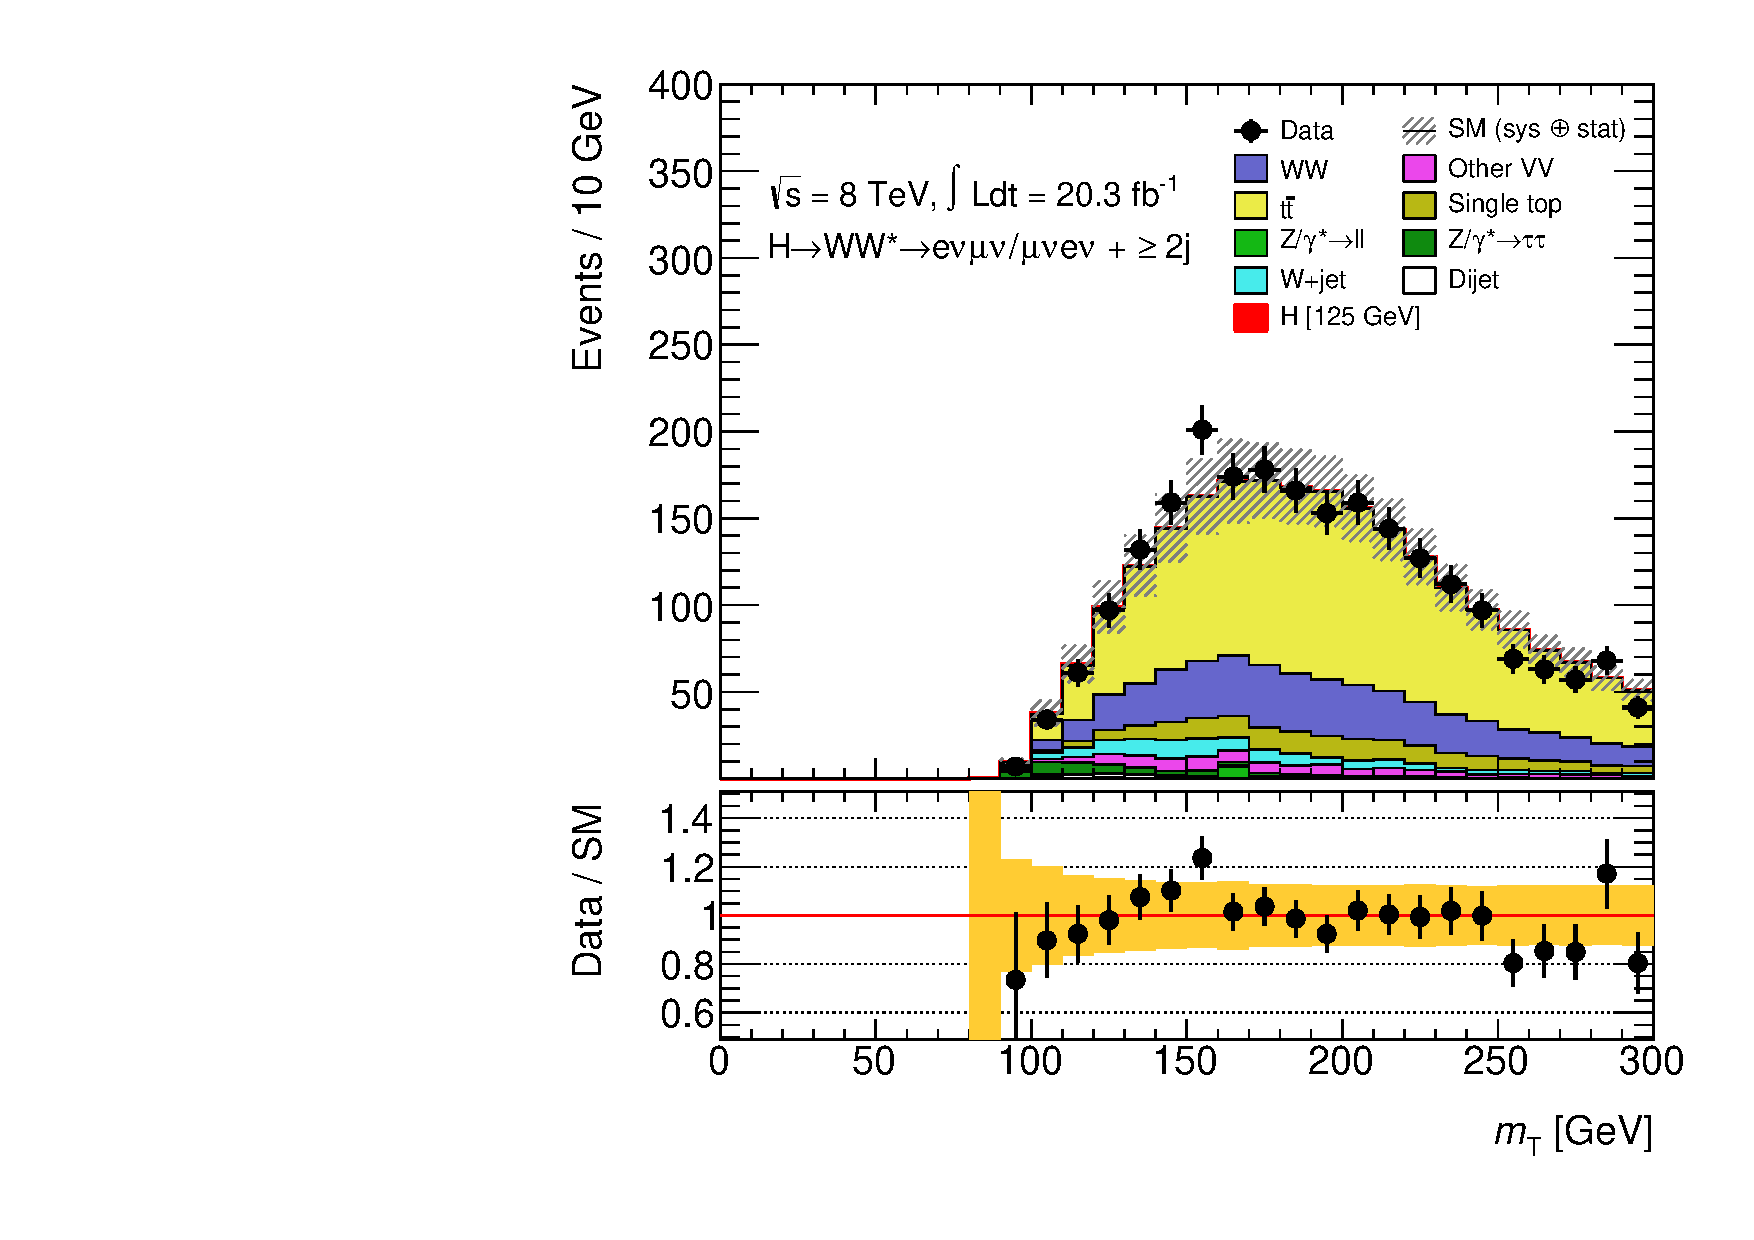
\includegraphics[width=0.495\textwidth]{tex/backgrounds/emme_CutFailVBFHighMllTopCR_2jetincl_MT_TrackHWW_Clj_mh125_lin}
	\hfill
	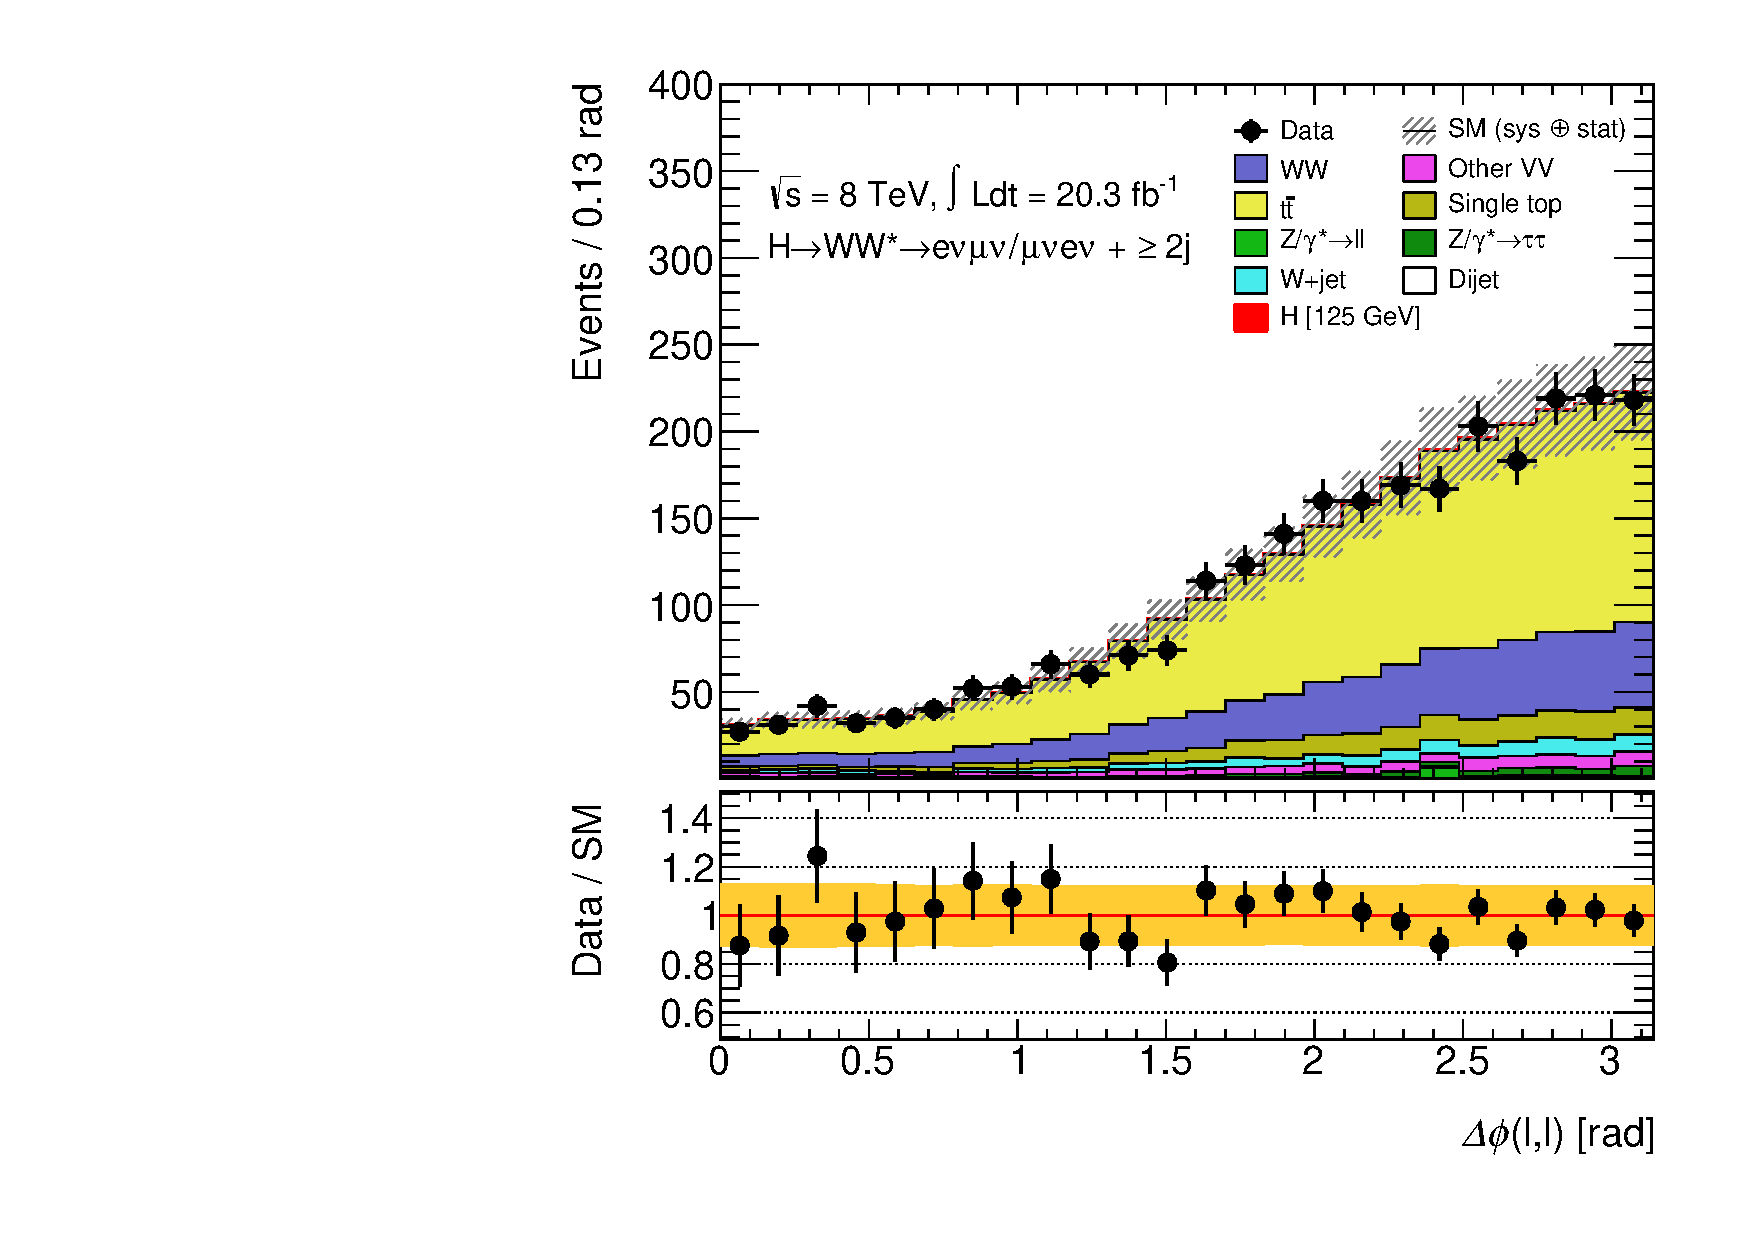
\includegraphics[width=0.495\textwidth]{tex/backgrounds/emme_CutFailVBFHighMllTopCR_2jetincl_DPhill_mh125_lin}
	\caption{The \mt (left) and \dphill (right) distributions in the top control region of 
	the \twojet bin. Normalisation factors are applied.}
	\label{fig:top:2j}
\end{figure}

To estimate the top background in \twojet regions other than the SR, the method is viewed 
as providing a simple data-driven normalisation factor. This is equivalent to neglecting 
the extrapolation uncertainties, but is helpful when plotting observables. The 
normalisation factor is measured to be \stat{1.078}{0.030}\todo{update}. 
\Figure~\ref{fig:top:2j} shows the good description of experimental data in the CR, 
after application of the normalisation factors.

